\documentclass[1p]{elsarticle_modified}
%\bibliographystyle{elsarticle-num}

%\usepackage[colorlinks]{hyperref}
%\usepackage{abbrmath_seonhwa} %\Abb, \Ascr, \Acal ,\Abf, \Afrak
\usepackage{amsfonts}
\usepackage{amssymb}
\usepackage{amsmath}
\usepackage{amsthm}
\usepackage{scalefnt}
\usepackage{amsbsy}
\usepackage{kotex}
\usepackage{caption}
\usepackage{subfig}
\usepackage{color}
\usepackage{graphicx}
\usepackage{xcolor} %% white, black, red, green, blue, cyan, magenta, yellow
\usepackage{float}
\usepackage{setspace}
\usepackage{hyperref}

\usepackage{tikz}
\usetikzlibrary{arrows}

\usepackage{multirow}
\usepackage{array} % fixed length table
\usepackage{hhline}

%%%%%%%%%%%%%%%%%%%%%
\makeatletter
\renewcommand*\env@matrix[1][\arraystretch]{%
	\edef\arraystretch{#1}%
	\hskip -\arraycolsep
	\let\@ifnextchar\new@ifnextchar
	\array{*\c@MaxMatrixCols c}}
\makeatother %https://tex.stackexchange.com/questions/14071/how-can-i-increase-the-line-spacing-in-a-matrix
%%%%%%%%%%%%%%%

\usepackage[normalem]{ulem}

\newcommand{\msout}[1]{\ifmmode\text{\sout{\ensuremath{#1}}}\else\sout{#1}\fi}
%SOURCE: \msout is \stkout macro in https://tex.stackexchange.com/questions/20609/strikeout-in-math-mode

\newcommand{\cancel}[1]{
	\ifmmode
	{\color{red}\msout{#1}}
	\else
	{\color{red}\sout{#1}}
	\fi
}

\newcommand{\add}[1]{
	{\color{blue}\uwave{#1}}
}

\newcommand{\replace}[2]{
	\ifmmode
	{\color{red}\msout{#1}}{\color{blue}\uwave{#2}}
	\else
	{\color{red}\sout{#1}}{\color{blue}\uwave{#2}}
	\fi
}

\newcommand{\Sol}{\mathcal{S}} %segment
\newcommand{\D}{D} %diagram
\newcommand{\A}{\mathcal{A}} %arc


%%%%%%%%%%%%%%%%%%%%%%%%%%%%%5 test

\def\sl{\operatorname{\textup{SL}}(2,\Cbb)}
\def\psl{\operatorname{\textup{PSL}}(2,\Cbb)}
\def\quan{\mkern 1mu \triangleright \mkern 1mu}

\theoremstyle{definition}
\newtheorem{thm}{Theorem}[section]
\newtheorem{prop}[thm]{Proposition}
\newtheorem{lem}[thm]{Lemma}
\newtheorem{ques}[thm]{Question}
\newtheorem{cor}[thm]{Corollary}
\newtheorem{defn}[thm]{Definition}
\newtheorem{exam}[thm]{Example}
\newtheorem{rmk}[thm]{Remark}
\newtheorem{alg}[thm]{Algorithm}

\newcommand{\I}{\sqrt{-1}}
\begin{document}

%\begin{frontmatter}
%
%\title{Boundary parabolic representations of knots up to 8 crossings}
%
%%% Group authors per affiliation:
%\author{Yunhi Cho} 
%\address{Department of Mathematics, University of Seoul, Seoul, Korea}
%\ead{yhcho@uos.ac.kr}
%
%
%\author{Seonhwa Kim} %\fnref{s_kim}}
%\address{Center for Geometry and Physics, Institute for Basic Science, Pohang, 37673, Korea}
%\ead{ryeona17@ibs.re.kr}
%
%\author{Hyuk Kim}
%\address{Department of Mathematical Sciences, Seoul National University, Seoul 08826, Korea}
%\ead{hyukkim@snu.ac.kr}
%
%\author{Seokbeom Yoon}
%\address{Department of Mathematical Sciences, Seoul National University, Seoul, 08826,  Korea}
%\ead{sbyoon15@snu.ac.kr}
%
%\begin{abstract}
%We find all boundary parabolic representation of knots up to 8 crossings.
%
%\end{abstract}
%\begin{keyword}
%    \MSC[2010] 57M25 
%\end{keyword}
%
%\end{frontmatter}

%\linenumbers
%\tableofcontents
%
\newcommand\colored[1]{\textcolor{white}{\rule[-0.35ex]{0.8em}{1.4ex}}\kern-0.8em\color{red} #1}%
%\newcommand\colored[1]{\textcolor{white}{ #1}\kern-2.17ex	\textcolor{white}{ #1}\kern-1.81ex	\textcolor{white}{ #1}\kern-2.15ex\color{red}#1	}

{\Large $\underline{12a_{0350}~(K12a_{0350})}$}

\setlength{\tabcolsep}{10pt}
\renewcommand{\arraystretch}{1.6}
\vspace{1cm}\begin{tabular}{m{100pt}>{\centering\arraybackslash}m{274pt}}
\multirow{5}{120pt}{
	\centering
	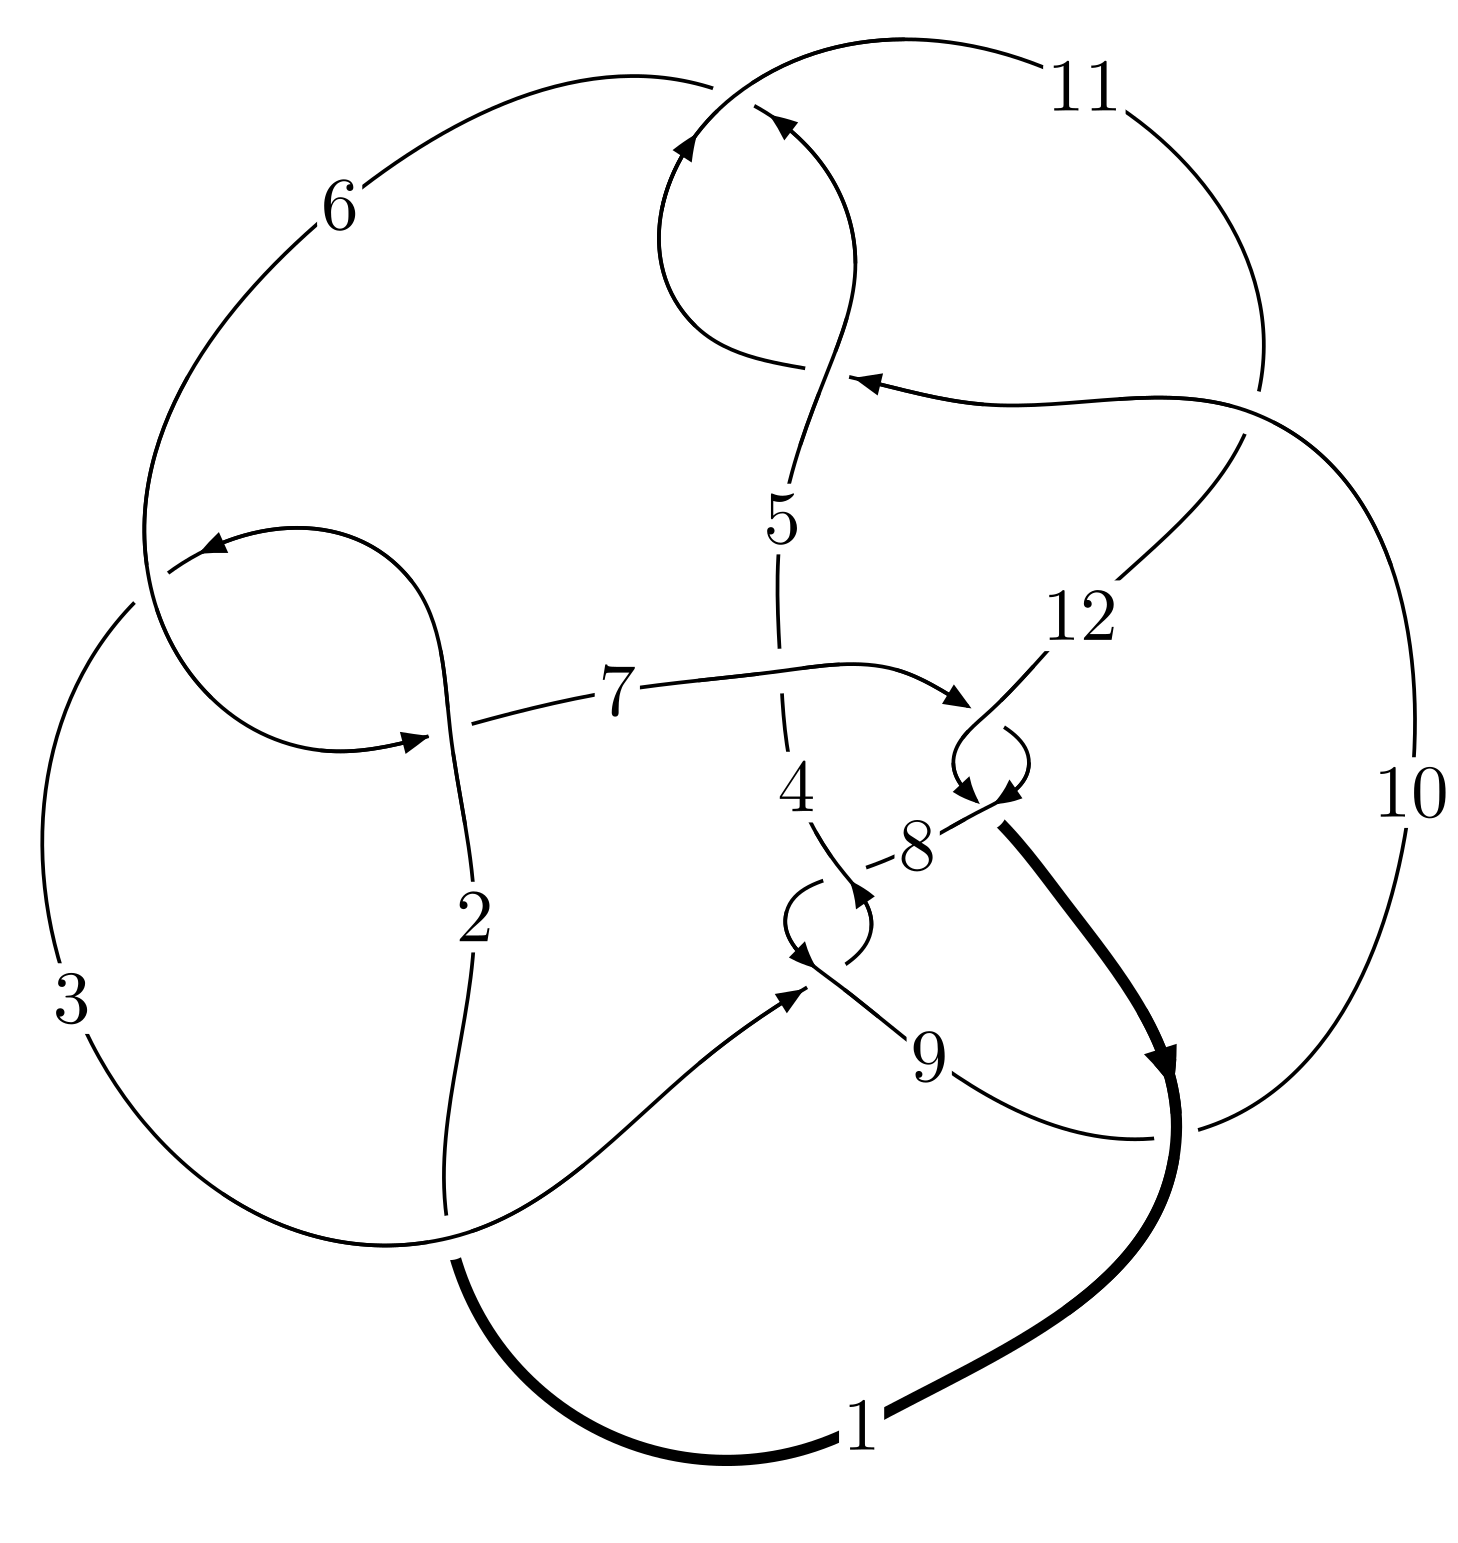
\includegraphics[width=112pt]{../../../GIT/diagram.site/Diagrams/png/1151_12a_0350.png}\\
\ \ \ A knot diagram\footnotemark}&
\allowdisplaybreaks
\textbf{Linearized knot diagam} \\
\cline{2-2}
 &
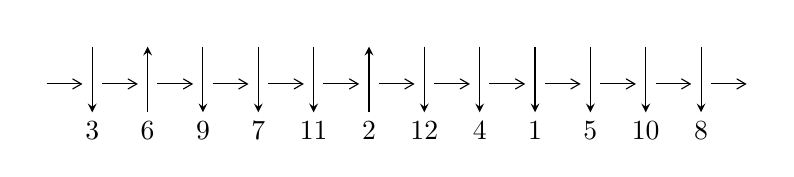
\begin{tikzpicture}[x=20pt, y=17pt]
	% nodes
	\node (C0) at (0, 0) {};
	\node (C1) at (1, 0) {};
	\node (C1U) at (1, +1) {};
	\node (C1D) at (1, -1) {3};

	\node (C2) at (2, 0) {};
	\node (C2U) at (2, +1) {};
	\node (C2D) at (2, -1) {6};

	\node (C3) at (3, 0) {};
	\node (C3U) at (3, +1) {};
	\node (C3D) at (3, -1) {9};

	\node (C4) at (4, 0) {};
	\node (C4U) at (4, +1) {};
	\node (C4D) at (4, -1) {7};

	\node (C5) at (5, 0) {};
	\node (C5U) at (5, +1) {};
	\node (C5D) at (5, -1) {11};

	\node (C6) at (6, 0) {};
	\node (C6U) at (6, +1) {};
	\node (C6D) at (6, -1) {2};

	\node (C7) at (7, 0) {};
	\node (C7U) at (7, +1) {};
	\node (C7D) at (7, -1) {12};

	\node (C8) at (8, 0) {};
	\node (C8U) at (8, +1) {};
	\node (C8D) at (8, -1) {4};

	\node (C9) at (9, 0) {};
	\node (C9U) at (9, +1) {};
	\node (C9D) at (9, -1) {1};

	\node (C10) at (10, 0) {};
	\node (C10U) at (10, +1) {};
	\node (C10D) at (10, -1) {5};

	\node (C11) at (11, 0) {};
	\node (C11U) at (11, +1) {};
	\node (C11D) at (11, -1) {10};

	\node (C12) at (12, 0) {};
	\node (C12U) at (12, +1) {};
	\node (C12D) at (12, -1) {8};
	\node (C13) at (13, 0) {};

	% arrows
	\draw[->,>={angle 60}]
	(C0) edge (C1) (C1) edge (C2) (C2) edge (C3) (C3) edge (C4) (C4) edge (C5) (C5) edge (C6) (C6) edge (C7) (C7) edge (C8) (C8) edge (C9) (C9) edge (C10) (C10) edge (C11) (C11) edge (C12) (C12) edge (C13) ;	\draw[->,>=stealth]
	(C1U) edge (C1D) (C2D) edge (C2U) (C3U) edge (C3D) (C4U) edge (C4D) (C5U) edge (C5D) (C6D) edge (C6U) (C7U) edge (C7D) (C8U) edge (C8D) (C9U) edge (C9D) (C10U) edge (C10D) (C11U) edge (C11D) (C12U) edge (C12D) ;
	\end{tikzpicture} \\
\hhline{~~} \\& 
\textbf{Solving Sequence} \\ \cline{2-2} 
 &
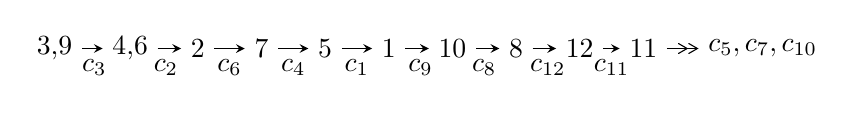
\begin{tikzpicture}[x=23pt, y=7pt]
	% node
	\node (A0) at (-1/8, 0) {3,9};
	\node (A1) at (17/16, 0) {4,6};
	\node (A2) at (17/8, 0) {2};
	\node (A3) at (25/8, 0) {7};
	\node (A4) at (33/8, 0) {5};
	\node (A5) at (41/8, 0) {1};
	\node (A6) at (49/8, 0) {10};
	\node (A7) at (57/8, 0) {8};
	\node (A8) at (65/8, 0) {12};
	\node (A9) at (73/8, 0) {11};
	\node (C1) at (1/2, -1) {$c_{3}$};
	\node (C2) at (13/8, -1) {$c_{2}$};
	\node (C3) at (21/8, -1) {$c_{6}$};
	\node (C4) at (29/8, -1) {$c_{4}$};
	\node (C5) at (37/8, -1) {$c_{1}$};
	\node (C6) at (45/8, -1) {$c_{9}$};
	\node (C7) at (53/8, -1) {$c_{8}$};
	\node (C8) at (61/8, -1) {$c_{12}$};
	\node (C9) at (69/8, -1) {$c_{11}$};
	\node (A10) at (11, 0) {$c_{5},c_{7},c_{10}$};

	% edge
	\draw[->,>=stealth]	
	(A0) edge (A1) (A1) edge (A2) (A2) edge (A3) (A3) edge (A4) (A4) edge (A5) (A5) edge (A6) (A6) edge (A7) (A7) edge (A8) (A8) edge (A9) ;
	\draw[->>,>={angle 60}]	
	(A9) edge (A10);
\end{tikzpicture} \\ 

\end{tabular} \\

\footnotetext{
The image of knot diagram is generated by the software ``\textbf{Draw programme}" developed by Andrew Bartholomew(\url{http://www.layer8.co.uk/maths/draw/index.htm\#Running-draw}), where we modified some parts for our purpose(\url{https://github.com/CATsTAILs/LinksPainter}).
}\phantom \\ \newline 
\centering \textbf{Ideals for irreducible components\footnotemark of $X_{\text{par}}$} 
 
\begin{align*}
I^u_{1}&=\langle 
-1.64650\times10^{477} u^{119}-2.04219\times10^{477} u^{118}+\cdots+5.37967\times10^{477} b+4.63499\times10^{477},\\
\phantom{I^u_{1}}&\phantom{= \langle  }-3.01914\times10^{477} u^{119}-5.15986\times10^{477} u^{118}+\cdots+1.39872\times10^{478} a-8.49918\times10^{477},\\
\phantom{I^u_{1}}&\phantom{= \langle  }u^{120}+u^{119}+\cdots+20 u-4\rangle \\
I^u_{2}&=\langle 
-3 a u+b-6 a-2 u-5,\;18 a^2-3 a u+30 a-4 u+15,\;u^2-2\rangle \\
\\
I^v_{1}&=\langle 
a,\;b- v,\;v^2+v+1\rangle \\
\end{align*}
\raggedright * 3 irreducible components of $\dim_{\mathbb{C}}=0$, with total 126 representations.\\
\footnotetext{All coefficients of polynomials are rational numbers. But the coefficients are sometimes approximated in decimal forms when there is not enough margin.}
\newpage
\renewcommand{\arraystretch}{1}
\centering \section*{I. $I^u_{1}= \langle -1.65\times10^{477} u^{119}-2.04\times10^{477} u^{118}+\cdots+5.38\times10^{477} b+4.63\times10^{477},\;-3.02\times10^{477} u^{119}-5.16\times10^{477} u^{118}+\cdots+1.40\times10^{478} a-8.50\times10^{477},\;u^{120}+u^{119}+\cdots+20 u-4 \rangle$}
\flushleft \textbf{(i) Arc colorings}\\
\begin{tabular}{m{7pt} m{180pt} m{7pt} m{180pt} }
\flushright $a_{3}=$&$\begin{pmatrix}1\\0\end{pmatrix}$ \\
\flushright $a_{9}=$&$\begin{pmatrix}0\\u\end{pmatrix}$ \\
\flushright $a_{4}=$&$\begin{pmatrix}1\\u^2\end{pmatrix}$ \\
\flushright $a_{6}=$&$\begin{pmatrix}0.215851 u^{119}+0.368900 u^{118}+\cdots-7.05008 u+0.607642\\0.306060 u^{119}+0.379613 u^{118}+\cdots+5.50411 u-0.861574\end{pmatrix}$ \\
\flushright $a_{2}=$&$\begin{pmatrix}-0.332303 u^{119}-0.00324083 u^{118}+\cdots+13.9294 u+1.86986\\0.0130671 u^{119}-0.181215 u^{118}+\cdots-8.87043 u+1.39199\end{pmatrix}$ \\
\flushright $a_{7}=$&$\begin{pmatrix}1.04132 u^{119}+1.06701 u^{118}+\cdots-15.4491 u+4.99065\\-0.237104 u^{119}-0.338198 u^{118}+\cdots+5.15503 u-0.569560\end{pmatrix}$ \\
\flushright $a_{5}=$&$\begin{pmatrix}-0.224721 u^{119}+0.373611 u^{118}+\cdots+35.9761 u-7.40116\\0.00695986 u^{119}+0.265753 u^{118}+\cdots+10.9571 u-2.73290\end{pmatrix}$ \\
\flushright $a_{1}=$&$\begin{pmatrix}-0.319236 u^{119}-0.184456 u^{118}+\cdots+5.05899 u+3.26185\\0.0130671 u^{119}-0.181215 u^{118}+\cdots-8.87043 u+1.39199\end{pmatrix}$ \\
\flushright $a_{10}=$&$\begin{pmatrix}-1.29087 u^{119}-0.889115 u^{118}+\cdots+28.2364 u-6.80811\\-0.0403642 u^{119}+0.0496315 u^{118}+\cdots+0.215259 u+0.360299\end{pmatrix}$ \\
\flushright $a_{8}=$&$\begin{pmatrix}u\\u^3+u\end{pmatrix}$ \\
\flushright $a_{12}=$&$\begin{pmatrix}-0.476243 u^{119}-0.238640 u^{118}+\cdots+10.5808 u+2.24891\\-0.0571666 u^{119}-0.190125 u^{118}+\cdots-6.03312 u+0.790341\end{pmatrix}$ \\
\flushright $a_{11}=$&$\begin{pmatrix}-0.281956 u^{119}+0.848688 u^{118}+\cdots+44.4292 u-6.63066\\0.0206301 u^{119}+0.0726329 u^{118}+\cdots-0.388572 u+0.172894\end{pmatrix}$\\&\end{tabular}
\flushleft \textbf{(ii) Obstruction class $= -1$}\\~\\
\flushleft \textbf{(iii) Cusp Shapes $= 0.797956 u^{119}+1.82037 u^{118}+\cdots+33.6708 u-21.8023$}\\~\\
\newpage\renewcommand{\arraystretch}{1}
\flushleft \textbf{(iv) u-Polynomials at the component}\newline \\
\begin{tabular}{m{50pt}|m{274pt}}
Crossings & \hspace{64pt}u-Polynomials at each crossing \\
\hline $$\begin{aligned}c_{1}\end{aligned}$$&$\begin{aligned}
&u^{120}+44 u^{119}+\cdots-3756 u+289
\end{aligned}$\\
\hline $$\begin{aligned}c_{2},c_{6}\end{aligned}$$&$\begin{aligned}
&u^{120}-2 u^{119}+\cdots+64 u+17
\end{aligned}$\\
\hline $$\begin{aligned}c_{3},c_{8}\end{aligned}$$&$\begin{aligned}
&u^{120}+u^{119}+\cdots+20 u-4
\end{aligned}$\\
\hline $$\begin{aligned}c_{4}\end{aligned}$$&$\begin{aligned}
&28561(28561 u^{120}+43940 u^{119}+\cdots-1.49875\times10^{8} u+1.98894\times10^{7})
\end{aligned}$\\
\hline $$\begin{aligned}c_{5},c_{10}\end{aligned}$$&$\begin{aligned}
&u^{120}+u^{119}+\cdots-36 u-4
\end{aligned}$\\
\hline $$\begin{aligned}c_{7},c_{12}\end{aligned}$$&$\begin{aligned}
&u^{120}+3 u^{119}+\cdots-495 u-343
\end{aligned}$\\
\hline $$\begin{aligned}c_{9}\end{aligned}$$&$\begin{aligned}
&28561(28561 u^{120}+160381 u^{119}+\cdots-9126759 u-5810977)
\end{aligned}$\\
\hline $$\begin{aligned}c_{11}\end{aligned}$$&$\begin{aligned}
&u^{120}+55 u^{119}+\cdots+208 u+16
\end{aligned}$\\
\hline
\end{tabular}\\~\\
\newpage\renewcommand{\arraystretch}{1}
\flushleft \textbf{(v) Riley Polynomials at the component}\newline \\
\begin{tabular}{m{50pt}|m{274pt}}
Crossings & \hspace{64pt}Riley Polynomials at each crossing \\
\hline $$\begin{aligned}c_{1}\end{aligned}$$&$\begin{aligned}
&y^{120}+68 y^{119}+\cdots-12388564 y+83521
\end{aligned}$\\
\hline $$\begin{aligned}c_{2},c_{6}\end{aligned}$$&$\begin{aligned}
&y^{120}+44 y^{119}+\cdots-3756 y+289
\end{aligned}$\\
\hline $$\begin{aligned}c_{3},c_{8}\end{aligned}$$&$\begin{aligned}
&y^{120}+65 y^{119}+\cdots+176 y+16
\end{aligned}$\\
\hline $$\begin{aligned}c_{4}\end{aligned}$$&$\begin{aligned}
&815730721\\
&\cdot(8.16\times10^{8} y^{120}+3.97\times10^{10} y^{119}+\cdots-1.14\times10^{16} y+3.96\times10^{14})
\end{aligned}$\\
\hline $$\begin{aligned}c_{5},c_{10}\end{aligned}$$&$\begin{aligned}
&y^{120}-55 y^{119}+\cdots-208 y+16
\end{aligned}$\\
\hline $$\begin{aligned}c_{7},c_{12}\end{aligned}$$&$\begin{aligned}
&y^{120}-69 y^{119}+\cdots-633301 y+117649
\end{aligned}$\\
\hline $$\begin{aligned}c_{9}\end{aligned}$$&$\begin{aligned}
&815730721\\
&\cdot(8.16\times10^{8} y^{120}+1.20\times10^{10} y^{119}+\cdots-3.67\times10^{14} y+3.38\times10^{13})
\end{aligned}$\\
\hline $$\begin{aligned}c_{11}\end{aligned}$$&$\begin{aligned}
&y^{120}+25 y^{119}+\cdots-26880 y+256
\end{aligned}$\\
\hline
\end{tabular}\\~\\
\newpage\flushleft \textbf{(vi) Complex Volumes and Cusp Shapes}
$$\begin{array}{c|c|c}  
\text{Solutions to }I^u_{1}& \I (\text{vol} + \sqrt{-1}CS) & \text{Cusp shape}\\
 \hline 
\begin{aligned}
u &= \phantom{-}0.202989 + 0.990498 I \\
a &= \phantom{-}1.83289 - 0.71222 I \\
b &= -0.954993 + 0.764552 I\end{aligned}
 & -0.32290 - 2.49959 I & \phantom{-0.000000 } 0 \\ \hline\begin{aligned}
u &= \phantom{-}0.202989 - 0.990498 I \\
a &= \phantom{-}1.83289 + 0.71222 I \\
b &= -0.954993 - 0.764552 I\end{aligned}
 & -0.32290 + 2.49959 I & \phantom{-0.000000 } 0 \\ \hline\begin{aligned}
u &= \phantom{-}0.125340 + 0.971618 I \\
a &= \phantom{-}2.29726 - 1.15154 I \\
b &= -0.720096 + 0.848381 I\end{aligned}
 & -0.16867 - 2.70921 I & \phantom{-0.000000 } 0 \\ \hline\begin{aligned}
u &= \phantom{-}0.125340 - 0.971618 I \\
a &= \phantom{-}2.29726 + 1.15154 I \\
b &= -0.720096 - 0.848381 I\end{aligned}
 & -0.16867 + 2.70921 I & \phantom{-0.000000 } 0 \\ \hline\begin{aligned}
u &= -0.215875 + 0.921340 I \\
a &= -2.05386 - 0.66138 I \\
b &= \phantom{-}0.97482 + 1.02658 I\end{aligned}
 & -1.27200 + 6.24574 I & \phantom{-0.000000 } 0 \\ \hline\begin{aligned}
u &= -0.215875 - 0.921340 I \\
a &= -2.05386 + 0.66138 I \\
b &= \phantom{-}0.97482 - 1.02658 I\end{aligned}
 & -1.27200 - 6.24574 I & \phantom{-0.000000 } 0 \\ \hline\begin{aligned}
u &= \phantom{-}1.067700 + 0.000614 I \\
a &= \phantom{-}0.699094 + 0.164069 I \\
b &= -0.790349 + 0.550536 I\end{aligned}
 & -0.94837 + 7.62370 I & \phantom{-0.000000 } 0 \\ \hline\begin{aligned}
u &= \phantom{-}1.067700 - 0.000614 I \\
a &= \phantom{-}0.699094 - 0.164069 I \\
b &= -0.790349 - 0.550536 I\end{aligned}
 & -0.94837 - 7.62370 I & \phantom{-0.000000 } 0 \\ \hline\begin{aligned}
u &= \phantom{-}0.147019 + 1.070360 I \\
a &= \phantom{-}1.49597 + 0.11383 I \\
b &= \phantom{-}0.387476 + 0.924439 I\end{aligned}
 & \phantom{-}0.041800 + 0.517074 I & \phantom{-0.000000 } 0 \\ \hline\begin{aligned}
u &= \phantom{-}0.147019 - 1.070360 I \\
a &= \phantom{-}1.49597 - 0.11383 I \\
b &= \phantom{-}0.387476 - 0.924439 I\end{aligned}
 & \phantom{-}0.041800 - 0.517074 I & \phantom{-0.000000 } 0\\
 \hline 
 \end{array}$$\newpage$$\begin{array}{c|c|c}  
\text{Solutions to }I^u_{1}& \I (\text{vol} + \sqrt{-1}CS) & \text{Cusp shape}\\
 \hline 
\begin{aligned}
u &= -0.852150 + 0.335345 I \\
a &= \phantom{-}0.862162 - 0.729618 I \\
b &= \phantom{-}0.007238 - 1.142000 I\end{aligned}
 & -6.79846 - 6.21229 I & \phantom{-0.000000 } 0 \\ \hline\begin{aligned}
u &= -0.852150 - 0.335345 I \\
a &= \phantom{-}0.862162 + 0.729618 I \\
b &= \phantom{-}0.007238 + 1.142000 I\end{aligned}
 & -6.79846 + 6.21229 I & \phantom{-0.000000 } 0 \\ \hline\begin{aligned}
u &= \phantom{-}0.914607\phantom{ +0.000000I} \\
a &= \phantom{-}0.851655\phantom{ +0.000000I} \\
b &= -0.435552\phantom{ +0.000000I}\end{aligned}
 & -5.82465\phantom{ +0.000000I} & \phantom{-0.000000 } 0 \\ \hline\begin{aligned}
u &= \phantom{-}0.780664 + 0.465076 I \\
a &= -1.096220 - 0.807047 I \\
b &= -0.008377 - 0.989825 I\end{aligned}
 & -4.16799 + 1.47675 I & \phantom{-0.000000 } 0 \\ \hline\begin{aligned}
u &= \phantom{-}0.780664 - 0.465076 I \\
a &= -1.096220 + 0.807047 I \\
b &= -0.008377 + 0.989825 I\end{aligned}
 & -4.16799 - 1.47675 I & \phantom{-0.000000 } 0 \\ \hline\begin{aligned}
u &= -0.887719 + 0.193758 I \\
a &= -0.588745 + 0.560769 I \\
b &= \phantom{-}0.650690 + 0.951781 I\end{aligned}
 & \phantom{-}2.29091 + 2.82384 I & \phantom{-0.000000 } 0 \\ \hline\begin{aligned}
u &= -0.887719 - 0.193758 I \\
a &= -0.588745 - 0.560769 I \\
b &= \phantom{-}0.650690 - 0.951781 I\end{aligned}
 & \phantom{-}2.29091 - 2.82384 I & \phantom{-0.000000 } 0 \\ \hline\begin{aligned}
u &= \phantom{-}0.240892 + 1.065480 I \\
a &= -0.498725 + 0.703933 I \\
b &= -0.317623 - 0.022486 I\end{aligned}
 & \phantom{-}1.14757 + 2.11836 I & \phantom{-0.000000 } 0 \\ \hline\begin{aligned}
u &= \phantom{-}0.240892 - 1.065480 I \\
a &= -0.498725 - 0.703933 I \\
b &= -0.317623 + 0.022486 I\end{aligned}
 & \phantom{-}1.14757 - 2.11836 I & \phantom{-0.000000 } 0 \\ \hline\begin{aligned}
u &= \phantom{-}0.290138 + 0.858508 I \\
a &= -0.03373 - 2.51112 I \\
b &= \phantom{-}0.281653 - 0.886609 I\end{aligned}
 & -0.31268 - 4.67708 I & \phantom{-0.000000 } 0\\
 \hline 
 \end{array}$$\newpage$$\begin{array}{c|c|c}  
\text{Solutions to }I^u_{1}& \I (\text{vol} + \sqrt{-1}CS) & \text{Cusp shape}\\
 \hline 
\begin{aligned}
u &= \phantom{-}0.290138 - 0.858508 I \\
a &= -0.03373 + 2.51112 I \\
b &= \phantom{-}0.281653 + 0.886609 I\end{aligned}
 & -0.31268 + 4.67708 I & \phantom{-0.000000 } 0 \\ \hline\begin{aligned}
u &= \phantom{-}0.258264 + 1.075510 I \\
a &= \phantom{-}1.50891 - 0.07679 I \\
b &= -1.143560 + 0.311585 I\end{aligned}
 & \phantom{-}1.67115 - 7.31624 I & \phantom{-0.000000 } 0 \\ \hline\begin{aligned}
u &= \phantom{-}0.258264 - 1.075510 I \\
a &= \phantom{-}1.50891 + 0.07679 I \\
b &= -1.143560 - 0.311585 I\end{aligned}
 & \phantom{-}1.67115 + 7.31624 I & \phantom{-0.000000 } 0 \\ \hline\begin{aligned}
u &= \phantom{-}0.764474 + 0.461851 I \\
a &= -0.298629 + 0.362400 I \\
b &= \phantom{-}0.670058 + 0.722219 I\end{aligned}
 & \phantom{-}2.98659 + 2.31380 I & \phantom{-0.000000 } 0 \\ \hline\begin{aligned}
u &= \phantom{-}0.764474 - 0.461851 I \\
a &= -0.298629 - 0.362400 I \\
b &= \phantom{-}0.670058 - 0.722219 I\end{aligned}
 & \phantom{-}2.98659 - 2.31380 I & \phantom{-0.000000 } 0 \\ \hline\begin{aligned}
u &= -0.160215 + 0.875406 I \\
a &= -0.178043 + 0.956426 I \\
b &= \phantom{-}0.237759 + 0.257881 I\end{aligned}
 & \phantom{-}1.78046 + 2.19670 I & \phantom{-0.000000 } 0 \\ \hline\begin{aligned}
u &= -0.160215 - 0.875406 I \\
a &= -0.178043 - 0.956426 I \\
b &= \phantom{-}0.237759 - 0.257881 I\end{aligned}
 & \phantom{-}1.78046 - 2.19670 I & \phantom{-0.000000 } 0 \\ \hline\begin{aligned}
u &= -1.115540 + 0.028792 I \\
a &= -0.719250 + 0.216715 I \\
b &= \phantom{-}0.717128 + 0.648150 I\end{aligned}
 & \phantom{-}0.99396 - 1.73965 I & \phantom{-0.000000 } 0 \\ \hline\begin{aligned}
u &= -1.115540 - 0.028792 I \\
a &= -0.719250 - 0.216715 I \\
b &= \phantom{-}0.717128 - 0.648150 I\end{aligned}
 & \phantom{-}0.99396 + 1.73965 I & \phantom{-0.000000 } 0 \\ \hline\begin{aligned}
u &= -0.240281 + 1.106510 I \\
a &= -1.232710 + 0.037129 I \\
b &= \phantom{-}0.996617 + 0.162947 I\end{aligned}
 & \phantom{-}2.78737 + 2.78465 I & \phantom{-0.000000 } 0\\
 \hline 
 \end{array}$$\newpage$$\begin{array}{c|c|c}  
\text{Solutions to }I^u_{1}& \I (\text{vol} + \sqrt{-1}CS) & \text{Cusp shape}\\
 \hline 
\begin{aligned}
u &= -0.240281 - 1.106510 I \\
a &= -1.232710 - 0.037129 I \\
b &= \phantom{-}0.996617 - 0.162947 I\end{aligned}
 & \phantom{-}2.78737 - 2.78465 I & \phantom{-0.000000 } 0 \\ \hline\begin{aligned}
u &= -0.185554 + 1.130230 I \\
a &= -0.482242 + 0.322174 I \\
b &= \phantom{-}0.564824 + 0.004451 I\end{aligned}
 & \phantom{-}2.28964 + 2.10386 I & \phantom{-0.000000 } 0 \\ \hline\begin{aligned}
u &= -0.185554 - 1.130230 I \\
a &= -0.482242 - 0.322174 I \\
b &= \phantom{-}0.564824 - 0.004451 I\end{aligned}
 & \phantom{-}2.28964 - 2.10386 I & \phantom{-0.000000 } 0 \\ \hline\begin{aligned}
u &= \phantom{-}0.845851 + 0.117669 I \\
a &= \phantom{-}0.432782 + 0.605481 I \\
b &= -0.643954 + 1.038350 I\end{aligned}
 & \phantom{-}0.98227 - 8.35275 I & \phantom{-0.000000 } 0 \\ \hline\begin{aligned}
u &= \phantom{-}0.845851 - 0.117669 I \\
a &= \phantom{-}0.432782 - 0.605481 I \\
b &= -0.643954 - 1.038350 I\end{aligned}
 & \phantom{-}0.98227 + 8.35275 I & \phantom{-0.000000 } 0 \\ \hline\begin{aligned}
u &= -0.171786 + 0.834696 I \\
a &= -1.92251 - 0.56569 I \\
b &= \phantom{-}0.729359 + 1.199970 I\end{aligned}
 & -2.12298 + 0.96742 I & \phantom{-0.000000 } 0 \\ \hline\begin{aligned}
u &= -0.171786 - 0.834696 I \\
a &= -1.92251 + 0.56569 I \\
b &= \phantom{-}0.729359 - 1.199970 I\end{aligned}
 & -2.12298 - 0.96742 I & \phantom{-0.000000 } 0 \\ \hline\begin{aligned}
u &= -1.034480 + 0.561437 I \\
a &= \phantom{-}1.085660 - 0.500482 I \\
b &= -0.207120 - 0.980921 I\end{aligned}
 & -8.61583 + 2.18923 I & \phantom{-0.000000 } 0 \\ \hline\begin{aligned}
u &= -1.034480 - 0.561437 I \\
a &= \phantom{-}1.085660 + 0.500482 I \\
b &= -0.207120 + 0.980921 I\end{aligned}
 & -8.61583 - 2.18923 I & \phantom{-0.000000 } 0 \\ \hline\begin{aligned}
u &= \phantom{-}0.509258 + 1.080060 I \\
a &= -0.693221 - 0.384489 I \\
b &= \phantom{-}0.161413 - 1.188380 I\end{aligned}
 & -2.20069 - 6.31530 I & \phantom{-0.000000 } 0\\
 \hline 
 \end{array}$$\newpage$$\begin{array}{c|c|c}  
\text{Solutions to }I^u_{1}& \I (\text{vol} + \sqrt{-1}CS) & \text{Cusp shape}\\
 \hline 
\begin{aligned}
u &= \phantom{-}0.509258 - 1.080060 I \\
a &= -0.693221 + 0.384489 I \\
b &= \phantom{-}0.161413 + 1.188380 I\end{aligned}
 & -2.20069 + 6.31530 I & \phantom{-0.000000 } 0 \\ \hline\begin{aligned}
u &= -1.200420 + 0.103729 I \\
a &= \phantom{-}0.773407 + 0.381234 I \\
b &= -0.665350 + 1.057800 I\end{aligned}
 & -2.44940 - 13.11410 I & \phantom{-0.000000 } 0 \\ \hline\begin{aligned}
u &= -1.200420 - 0.103729 I \\
a &= \phantom{-}0.773407 - 0.381234 I \\
b &= -0.665350 - 1.057800 I\end{aligned}
 & -2.44940 + 13.11410 I & \phantom{-0.000000 } 0 \\ \hline\begin{aligned}
u &= -0.616678 + 1.060240 I \\
a &= \phantom{-}0.185913 - 0.231296 I \\
b &= \phantom{-}0.017347 - 1.145710 I\end{aligned}
 & -6.86455 + 3.65797 I & \phantom{-0.000000 } 0 \\ \hline\begin{aligned}
u &= -0.616678 - 1.060240 I \\
a &= \phantom{-}0.185913 + 0.231296 I \\
b &= \phantom{-}0.017347 + 1.145710 I\end{aligned}
 & -6.86455 - 3.65797 I & \phantom{-0.000000 } 0 \\ \hline\begin{aligned}
u &= \phantom{-}0.071139 + 0.767821 I \\
a &= -0.766900 + 0.278980 I \\
b &= \phantom{-}0.414325 + 1.037240 I\end{aligned}
 & -0.71039 + 1.36487 I & -6.45479 + 0. I\phantom{ +0.000000I} \\ \hline\begin{aligned}
u &= \phantom{-}0.071139 - 0.767821 I \\
a &= -0.766900 - 0.278980 I \\
b &= \phantom{-}0.414325 - 1.037240 I\end{aligned}
 & -0.71039 - 1.36487 I & -6.45479 + 0. I\phantom{ +0.000000I} \\ \hline\begin{aligned}
u &= \phantom{-}1.225120 + 0.196206 I \\
a &= -0.734550 + 0.348848 I \\
b &= \phantom{-}0.663880 + 0.999341 I\end{aligned}
 & -0.04980 + 7.04998 I & \phantom{-0.000000 } 0 \\ \hline\begin{aligned}
u &= \phantom{-}1.225120 - 0.196206 I \\
a &= -0.734550 - 0.348848 I \\
b &= \phantom{-}0.663880 - 0.999341 I\end{aligned}
 & -0.04980 - 7.04998 I & \phantom{-0.000000 } 0 \\ \hline\begin{aligned}
u &= -0.527948 + 1.123740 I \\
a &= \phantom{-}0.720724 - 0.101032 I \\
b &= -0.139915 - 1.287900 I\end{aligned}
 & -4.36117 + 11.26390 I & \phantom{-0.000000 } 0\\
 \hline 
 \end{array}$$\newpage$$\begin{array}{c|c|c}  
\text{Solutions to }I^u_{1}& \I (\text{vol} + \sqrt{-1}CS) & \text{Cusp shape}\\
 \hline 
\begin{aligned}
u &= -0.527948 - 1.123740 I \\
a &= \phantom{-}0.720724 + 0.101032 I \\
b &= -0.139915 + 1.287900 I\end{aligned}
 & -4.36117 - 11.26390 I & \phantom{-0.000000 } 0 \\ \hline\begin{aligned}
u &= \phantom{-}0.040199 + 1.251880 I \\
a &= -0.974076 - 0.823210 I \\
b &= -0.177940 + 0.691389 I\end{aligned}
 & -0.72258 - 3.71661 I & \phantom{-0.000000 } 0 \\ \hline\begin{aligned}
u &= \phantom{-}0.040199 - 1.251880 I \\
a &= -0.974076 + 0.823210 I \\
b &= -0.177940 - 0.691389 I\end{aligned}
 & -0.72258 + 3.71661 I & \phantom{-0.000000 } 0 \\ \hline\begin{aligned}
u &= \phantom{-}0.151062 + 0.722891 I \\
a &= \phantom{-}1.43814 - 0.59435 I \\
b &= -0.484144 + 1.294440 I\end{aligned}
 & -2.51414 - 4.12934 I & -16.4536 + 7.0812 I \\ \hline\begin{aligned}
u &= \phantom{-}0.151062 - 0.722891 I \\
a &= \phantom{-}1.43814 + 0.59435 I \\
b &= -0.484144 - 1.294440 I\end{aligned}
 & -2.51414 + 4.12934 I & -16.4536 - 7.0812 I \\ \hline\begin{aligned}
u &= -0.641582 + 0.334485 I \\
a &= \phantom{-}0.157238 + 0.522437 I \\
b &= -0.703427 + 0.562473 I\end{aligned}
 & \phantom{-}2.37369 + 3.13295 I & -5.19542 - 2.99721 I \\ \hline\begin{aligned}
u &= -0.641582 - 0.334485 I \\
a &= \phantom{-}0.157238 - 0.522437 I \\
b &= -0.703427 - 0.562473 I\end{aligned}
 & \phantom{-}2.37369 - 3.13295 I & -5.19542 + 2.99721 I \\ \hline\begin{aligned}
u &= -0.092146 + 1.281900 I \\
a &= -1.13710 + 1.04294 I \\
b &= \phantom{-}0.542386 - 0.612790 I\end{aligned}
 & \phantom{-}2.11803 + 1.48065 I & \phantom{-0.000000 } 0 \\ \hline\begin{aligned}
u &= -0.092146 - 1.281900 I \\
a &= -1.13710 - 1.04294 I \\
b &= \phantom{-}0.542386 + 0.612790 I\end{aligned}
 & \phantom{-}2.11803 - 1.48065 I & \phantom{-0.000000 } 0 \\ \hline\begin{aligned}
u &= -0.301148 + 1.254700 I \\
a &= -1.19267 + 0.79638 I \\
b &= \phantom{-}1.046590 - 0.593449 I\end{aligned}
 & \phantom{-}6.96547 + 6.35967 I & \phantom{-0.000000 } 0\\
 \hline 
 \end{array}$$\newpage$$\begin{array}{c|c|c}  
\text{Solutions to }I^u_{1}& \I (\text{vol} + \sqrt{-1}CS) & \text{Cusp shape}\\
 \hline 
\begin{aligned}
u &= -0.301148 - 1.254700 I \\
a &= -1.19267 - 0.79638 I \\
b &= \phantom{-}1.046590 + 0.593449 I\end{aligned}
 & \phantom{-}6.96547 - 6.35967 I & \phantom{-0.000000 } 0 \\ \hline\begin{aligned}
u &= -0.066911 + 0.696541 I \\
a &= -2.64854 - 2.78771 I \\
b &= -0.335906 - 0.774807 I\end{aligned}
 & -0.521713 - 0.088016 I & -14.1626 + 0.5129 I \\ \hline\begin{aligned}
u &= -0.066911 - 0.696541 I \\
a &= -2.64854 + 2.78771 I \\
b &= -0.335906 + 0.774807 I\end{aligned}
 & -0.521713 + 0.088016 I & -14.1626 - 0.5129 I \\ \hline\begin{aligned}
u &= \phantom{-}0.294325 + 1.288810 I \\
a &= \phantom{-}1.145480 + 0.813247 I \\
b &= -0.966050 - 0.664872 I\end{aligned}
 & \phantom{-}8.11911 - 1.05080 I & \phantom{-0.000000 } 0 \\ \hline\begin{aligned}
u &= \phantom{-}0.294325 - 1.288810 I \\
a &= \phantom{-}1.145480 - 0.813247 I \\
b &= -0.966050 + 0.664872 I\end{aligned}
 & \phantom{-}8.11911 + 1.05080 I & \phantom{-0.000000 } 0 \\ \hline\begin{aligned}
u &= \phantom{-}0.341475 + 1.280630 I \\
a &= -1.90105 - 0.00872 I \\
b &= \phantom{-}0.602369 - 1.033590 I\end{aligned}
 & \phantom{-}0.76201 - 6.19196 I & \phantom{-0.000000 } 0 \\ \hline\begin{aligned}
u &= \phantom{-}0.341475 - 1.280630 I \\
a &= -1.90105 + 0.00872 I \\
b &= \phantom{-}0.602369 + 1.033590 I\end{aligned}
 & \phantom{-}0.76201 + 6.19196 I & \phantom{-0.000000 } 0 \\ \hline\begin{aligned}
u &= -0.796395 + 1.099760 I \\
a &= -1.39317 + 0.55781 I \\
b &= \phantom{-}0.680943 + 0.865093 I\end{aligned}
 & \phantom{-}3.81397 + 2.16376 I & \phantom{-0.000000 } 0 \\ \hline\begin{aligned}
u &= -0.796395 - 1.099760 I \\
a &= -1.39317 - 0.55781 I \\
b &= \phantom{-}0.680943 - 0.865093 I\end{aligned}
 & \phantom{-}3.81397 - 2.16376 I & \phantom{-0.000000 } 0 \\ \hline\begin{aligned}
u &= \phantom{-}0.423195 + 1.291600 I \\
a &= -1.82406 + 0.03051 I \\
b &= \phantom{-}0.763275 - 1.134570 I\end{aligned}
 & \phantom{-}5.24553 - 12.87400 I & \phantom{-0.000000 } 0\\
 \hline 
 \end{array}$$\newpage$$\begin{array}{c|c|c}  
\text{Solutions to }I^u_{1}& \I (\text{vol} + \sqrt{-1}CS) & \text{Cusp shape}\\
 \hline 
\begin{aligned}
u &= \phantom{-}0.423195 - 1.291600 I \\
a &= -1.82406 - 0.03051 I \\
b &= \phantom{-}0.763275 + 1.134570 I\end{aligned}
 & \phantom{-}5.24553 + 12.87400 I & \phantom{-0.000000 } 0 \\ \hline\begin{aligned}
u &= -0.414925 + 1.307140 I \\
a &= \phantom{-}1.82897 + 0.01688 I \\
b &= -0.763150 - 1.074800 I\end{aligned}
 & \phantom{-}6.81555 + 7.35933 I & \phantom{-0.000000 } 0 \\ \hline\begin{aligned}
u &= -0.414925 - 1.307140 I \\
a &= \phantom{-}1.82897 - 0.01688 I \\
b &= -0.763150 + 1.074800 I\end{aligned}
 & \phantom{-}6.81555 - 7.35933 I & \phantom{-0.000000 } 0 \\ \hline\begin{aligned}
u &= \phantom{-}0.193170 + 0.594552 I \\
a &= \phantom{-}0.740458 - 0.666529 I \\
b &= -0.098240 + 1.240000 I\end{aligned}
 & -2.62261 + 1.47478 I & -15.3851 - 1.4664 I \\ \hline\begin{aligned}
u &= \phantom{-}0.193170 - 0.594552 I \\
a &= \phantom{-}0.740458 + 0.666529 I \\
b &= -0.098240 - 1.240000 I\end{aligned}
 & -2.62261 - 1.47478 I & -15.3851 + 1.4664 I \\ \hline\begin{aligned}
u &= \phantom{-}0.655153 + 1.238030 I \\
a &= -0.453361 - 0.509072 I \\
b &= \phantom{-}0.676490 + 0.837280 I\end{aligned}
 & \phantom{-}3.89800 + 3.07288 I & \phantom{-0.000000 } 0 \\ \hline\begin{aligned}
u &= \phantom{-}0.655153 - 1.238030 I \\
a &= -0.453361 + 0.509072 I \\
b &= \phantom{-}0.676490 - 0.837280 I\end{aligned}
 & \phantom{-}3.89800 - 3.07288 I & \phantom{-0.000000 } 0 \\ \hline\begin{aligned}
u &= -0.287460 + 0.509167 I \\
a &= -1.030630 + 0.288101 I \\
b &= \phantom{-}0.294151 + 0.891432 I\end{aligned}
 & -0.56479 + 1.45174 I & -5.69061 - 3.81457 I \\ \hline\begin{aligned}
u &= -0.287460 - 0.509167 I \\
a &= -1.030630 - 0.288101 I \\
b &= \phantom{-}0.294151 - 0.891432 I\end{aligned}
 & -0.56479 - 1.45174 I & -5.69061 + 3.81457 I \\ \hline\begin{aligned}
u &= -0.150834 + 0.552483 I \\
a &= \phantom{-}0.224663 - 0.926766 I \\
b &= -0.284188 + 1.222330 I\end{aligned}
 & -2.60685 + 1.42151 I & -15.3519 - 4.1761 I\\
 \hline 
 \end{array}$$\newpage$$\begin{array}{c|c|c}  
\text{Solutions to }I^u_{1}& \I (\text{vol} + \sqrt{-1}CS) & \text{Cusp shape}\\
 \hline 
\begin{aligned}
u &= -0.150834 - 0.552483 I \\
a &= \phantom{-}0.224663 + 0.926766 I \\
b &= -0.284188 - 1.222330 I\end{aligned}
 & -2.60685 - 1.42151 I & -15.3519 + 4.1761 I \\ \hline\begin{aligned}
u &= \phantom{-}0.52628 + 1.33490 I \\
a &= -0.952515 - 0.880427 I \\
b &= \phantom{-}0.959021 + 0.573110 I\end{aligned}
 & \phantom{-}3.19983 - 13.23160 I & \phantom{-0.000000 } 0 \\ \hline\begin{aligned}
u &= \phantom{-}0.52628 - 1.33490 I \\
a &= -0.952515 + 0.880427 I \\
b &= \phantom{-}0.959021 - 0.573110 I\end{aligned}
 & \phantom{-}3.19983 + 13.23160 I & \phantom{-0.000000 } 0 \\ \hline\begin{aligned}
u &= -0.53445 + 1.33597 I \\
a &= \phantom{-}0.888636 - 0.841711 I \\
b &= -0.909341 + 0.611982 I\end{aligned}
 & \phantom{-}5.11042 + 7.48156 I & \phantom{-0.000000 } 0 \\ \hline\begin{aligned}
u &= -0.53445 - 1.33597 I \\
a &= \phantom{-}0.888636 + 0.841711 I \\
b &= -0.909341 - 0.611982 I\end{aligned}
 & \phantom{-}5.11042 - 7.48156 I & \phantom{-0.000000 } 0 \\ \hline\begin{aligned}
u &= \phantom{-}0.74543 + 1.23902 I \\
a &= \phantom{-}1.57046 + 0.44108 I \\
b &= -0.703722 + 0.938834 I\end{aligned}
 & \phantom{-}4.89450 - 8.45588 I & \phantom{-0.000000 } 0 \\ \hline\begin{aligned}
u &= \phantom{-}0.74543 - 1.23902 I \\
a &= \phantom{-}1.57046 - 0.44108 I \\
b &= -0.703722 - 0.938834 I\end{aligned}
 & \phantom{-}4.89450 + 8.45588 I & \phantom{-0.000000 } 0 \\ \hline\begin{aligned}
u &= \phantom{-}0.551421 + 0.017870 I \\
a &= \phantom{-}0.19708 - 1.54303 I \\
b &= -0.397472 - 1.008780 I\end{aligned}
 & -3.11028 + 2.85114 I & -15.0953 - 5.2463 I \\ \hline\begin{aligned}
u &= \phantom{-}0.551421 - 0.017870 I \\
a &= \phantom{-}0.19708 + 1.54303 I \\
b &= -0.397472 + 1.008780 I\end{aligned}
 & -3.11028 - 2.85114 I & -15.0953 + 5.2463 I \\ \hline\begin{aligned}
u &= -0.39398 + 1.39456 I \\
a &= \phantom{-}1.74350 + 0.04414 I \\
b &= -0.712038 - 0.891443 I\end{aligned}
 & \phantom{-}5.99648 + 3.81310 I & \phantom{-0.000000 } 0\\
 \hline 
 \end{array}$$\newpage$$\begin{array}{c|c|c}  
\text{Solutions to }I^u_{1}& \I (\text{vol} + \sqrt{-1}CS) & \text{Cusp shape}\\
 \hline 
\begin{aligned}
u &= -0.39398 - 1.39456 I \\
a &= \phantom{-}1.74350 - 0.04414 I \\
b &= -0.712038 + 0.891443 I\end{aligned}
 & \phantom{-}5.99648 - 3.81310 I & \phantom{-0.000000 } 0 \\ \hline\begin{aligned}
u &= -0.60580 + 1.31894 I \\
a &= \phantom{-}0.637580 - 0.640539 I \\
b &= -0.739316 + 0.759070 I\end{aligned}
 & \phantom{-}5.43801 + 2.96205 I & \phantom{-0.000000 } 0 \\ \hline\begin{aligned}
u &= -0.60580 - 1.31894 I \\
a &= \phantom{-}0.637580 + 0.640539 I \\
b &= -0.739316 - 0.759070 I\end{aligned}
 & \phantom{-}5.43801 - 2.96205 I & \phantom{-0.000000 } 0 \\ \hline\begin{aligned}
u &= \phantom{-}0.52914 + 1.37088 I \\
a &= -0.941382 - 0.654409 I \\
b &= \phantom{-}0.754936 + 0.529073 I\end{aligned}
 & -1.28468 - 5.21244 I & \phantom{-0.000000 } 0 \\ \hline\begin{aligned}
u &= \phantom{-}0.52914 - 1.37088 I \\
a &= -0.941382 + 0.654409 I \\
b &= \phantom{-}0.754936 - 0.529073 I\end{aligned}
 & -1.28468 + 5.21244 I & \phantom{-0.000000 } 0 \\ \hline\begin{aligned}
u &= \phantom{-}0.24828 + 1.44950 I \\
a &= \phantom{-}1.118450 + 0.722661 I \\
b &= -0.731705 - 0.815881 I\end{aligned}
 & \phantom{-}6.22710 + 1.68218 I & \phantom{-0.000000 } 0 \\ \hline\begin{aligned}
u &= \phantom{-}0.24828 - 1.44950 I \\
a &= \phantom{-}1.118450 - 0.722661 I \\
b &= -0.731705 + 0.815881 I\end{aligned}
 & \phantom{-}6.22710 - 1.68218 I & \phantom{-0.000000 } 0 \\ \hline\begin{aligned}
u &= -0.59764 + 1.35597 I \\
a &= -1.89626 + 0.18431 I \\
b &= \phantom{-}0.727490 + 1.115030 I\end{aligned}
 & \phantom{-}1.5129 + 19.3967 I & \phantom{-0.000000 } 0 \\ \hline\begin{aligned}
u &= -0.59764 - 1.35597 I \\
a &= -1.89626 - 0.18431 I \\
b &= \phantom{-}0.727490 - 1.115030 I\end{aligned}
 & \phantom{-}1.5129 - 19.3967 I & \phantom{-0.000000 } 0 \\ \hline\begin{aligned}
u &= \phantom{-}0.62148 + 1.34536 I \\
a &= \phantom{-}1.84103 + 0.23572 I \\
b &= -0.725741 + 1.080140 I\end{aligned}
 & \phantom{-}3.66188 - 13.51110 I & \phantom{-0.000000 } 0\\
 \hline 
 \end{array}$$\newpage$$\begin{array}{c|c|c}  
\text{Solutions to }I^u_{1}& \I (\text{vol} + \sqrt{-1}CS) & \text{Cusp shape}\\
 \hline 
\begin{aligned}
u &= \phantom{-}0.62148 - 1.34536 I \\
a &= \phantom{-}1.84103 - 0.23572 I \\
b &= -0.725741 - 1.080140 I\end{aligned}
 & \phantom{-}3.66188 + 13.51110 I & \phantom{-0.000000 } 0 \\ \hline\begin{aligned}
u &= \phantom{-}0.45750 + 1.47072 I \\
a &= -1.59958 + 0.00596 I \\
b &= \phantom{-}0.683108 - 0.786787 I\end{aligned}
 & \phantom{-}3.66093 + 1.77132 I & \phantom{-0.000000 } 0 \\ \hline\begin{aligned}
u &= \phantom{-}0.45750 - 1.47072 I \\
a &= -1.59958 - 0.00596 I \\
b &= \phantom{-}0.683108 + 0.786787 I\end{aligned}
 & \phantom{-}3.66093 - 1.77132 I & \phantom{-0.000000 } 0 \\ \hline\begin{aligned}
u &= -0.427567 + 0.124510 I \\
a &= -1.27938 + 0.74577 I \\
b &= -0.520833 - 0.306625 I\end{aligned}
 & -0.410665 + 0.350990 I & -9.14009 - 0.28858 I \\ \hline\begin{aligned}
u &= -0.427567 - 0.124510 I \\
a &= -1.27938 - 0.74577 I \\
b &= -0.520833 + 0.306625 I\end{aligned}
 & -0.410665 - 0.350990 I & -9.14009 + 0.28858 I \\ \hline\begin{aligned}
u &= -0.67604 + 1.40424 I \\
a &= -1.68215 + 0.15655 I \\
b &= \phantom{-}0.650729 + 1.052630 I\end{aligned}
 & -2.80574 + 10.55840 I & \phantom{-0.000000 } 0 \\ \hline\begin{aligned}
u &= -0.67604 - 1.40424 I \\
a &= -1.68215 - 0.15655 I \\
b &= \phantom{-}0.650729 - 1.052630 I\end{aligned}
 & -2.80574 - 10.55840 I & \phantom{-0.000000 } 0 \\ \hline\begin{aligned}
u &= -1.54967 + 0.37438 I \\
a &= \phantom{-}0.769588 + 0.204123 I \\
b &= -0.577365 + 0.931964 I\end{aligned}
 & -6.61511 - 3.02974 I & \phantom{-0.000000 } 0 \\ \hline\begin{aligned}
u &= -1.54967 - 0.37438 I \\
a &= \phantom{-}0.769588 - 0.204123 I \\
b &= -0.577365 - 0.931964 I\end{aligned}
 & -6.61511 + 3.02974 I & \phantom{-0.000000 } 0 \\ \hline\begin{aligned}
u &= \phantom{-}1.60506 + 0.18152 I \\
a &= \phantom{-}0.884414 + 0.227938 I \\
b &= -0.545678 + 0.787014 I\end{aligned}
 & -6.11465 - 1.47265 I & \phantom{-0.000000 } 0\\
 \hline 
 \end{array}$$\newpage$$\begin{array}{c|c|c}  
\text{Solutions to }I^u_{1}& \I (\text{vol} + \sqrt{-1}CS) & \text{Cusp shape}\\
 \hline 
\begin{aligned}
u &= \phantom{-}1.60506 - 0.18152 I \\
a &= \phantom{-}0.884414 - 0.227938 I \\
b &= -0.545678 - 0.787014 I\end{aligned}
 & -6.11465 + 1.47265 I & \phantom{-0.000000 } 0 \\ \hline\begin{aligned}
u &= -0.33661 + 1.58852 I \\
a &= -1.030070 + 0.585576 I \\
b &= \phantom{-}0.672963 - 0.909232 I\end{aligned}
 & \phantom{-}3.28785 - 7.00671 I & \phantom{-0.000000 } 0 \\ \hline\begin{aligned}
u &= -0.33661 - 1.58852 I \\
a &= -1.030070 - 0.585576 I \\
b &= \phantom{-}0.672963 + 0.909232 I\end{aligned}
 & \phantom{-}3.28785 + 7.00671 I & \phantom{-0.000000 } 0 \\ \hline\begin{aligned}
u &= -0.373865\phantom{ +0.000000I} \\
a &= -0.539447\phantom{ +0.000000I} \\
b &= -0.335233\phantom{ +0.000000I}\end{aligned}
 & -0.794733\phantom{ +0.000000I} & -12.4810\phantom{ +0.000000I} \\ \hline\begin{aligned}
u &= \phantom{-}0.336296 + 0.040421 I \\
a &= \phantom{-}1.66344 + 1.98608 I \\
b &= \phantom{-}0.711214 - 0.564146 I\end{aligned}
 & -1.12664 - 4.84437 I & -10.81095 + 6.16099 I \\ \hline\begin{aligned}
u &= \phantom{-}0.336296 - 0.040421 I \\
a &= \phantom{-}1.66344 - 1.98608 I \\
b &= \phantom{-}0.711214 + 0.564146 I\end{aligned}
 & -1.12664 + 4.84437 I & -10.81095 - 6.16099 I \\ \hline\begin{aligned}
u &= -0.108600 + 0.306225 I \\
a &= \phantom{-}1.42426 - 2.32937 I \\
b &= -0.564521 + 1.107430 I\end{aligned}
 & -2.48368 - 3.99664 I & -14.3466 + 4.3294 I \\ \hline\begin{aligned}
u &= -0.108600 - 0.306225 I \\
a &= \phantom{-}1.42426 + 2.32937 I \\
b &= -0.564521 - 1.107430 I\end{aligned}
 & -2.48368 + 3.99664 I & -14.3466 - 4.3294 I \\ \hline\begin{aligned}
u &= \phantom{-}0.171725 + 0.147653 I \\
a &= -0.47354 - 4.27439 I \\
b &= \phantom{-}0.677264 + 0.943220 I\end{aligned}
 & -2.15402 + 0.44006 I & -13.51281 + 1.33837 I \\ \hline\begin{aligned}
u &= \phantom{-}0.171725 - 0.147653 I \\
a &= -0.47354 + 4.27439 I \\
b &= \phantom{-}0.677264 - 0.943220 I\end{aligned}
 & -2.15402 - 0.44006 I & -13.51281 - 1.33837 I\\
 \hline 
 \end{array}$$\newpage\newpage\renewcommand{\arraystretch}{1}
\centering \section*{II. $I^u_{2}= \langle -3 a u+b-6 a-2 u-5,\;18 a^2-3 a u+30 a-4 u+15,\;u^2-2 \rangle$}
\flushleft \textbf{(i) Arc colorings}\\
\begin{tabular}{m{7pt} m{180pt} m{7pt} m{180pt} }
\flushright $a_{3}=$&$\begin{pmatrix}1\\0\end{pmatrix}$ \\
\flushright $a_{9}=$&$\begin{pmatrix}0\\u\end{pmatrix}$ \\
\flushright $a_{4}=$&$\begin{pmatrix}1\\2\end{pmatrix}$ \\
\flushright $a_{6}=$&$\begin{pmatrix}a\\3 a u+6 a+2 u+5\end{pmatrix}$ \\
\flushright $a_{2}=$&$\begin{pmatrix}-2 a u-4 a-\frac{7}{6} u-\frac{8}{3}\\3 a u+6 a+2 u+4\end{pmatrix}$ \\
\flushright $a_{7}=$&$\begin{pmatrix}a u+2 a+\frac{5}{6} u+\frac{4}{3}\\3 a u+6 a+2 u+4\end{pmatrix}$ \\
\flushright $a_{5}=$&$\begin{pmatrix}-\frac{2}{3} a u- a-\frac{4}{9} u+\frac{1}{9}\\-3 a u-4 a-2 u-1\end{pmatrix}$ \\
\flushright $a_{1}=$&$\begin{pmatrix}a u+2 a+\frac{5}{6} u+\frac{4}{3}\\3 a u+6 a+2 u+4\end{pmatrix}$ \\
\flushright $a_{10}=$&$\begin{pmatrix}-\frac{2}{3} a+\frac{1}{18} u-\frac{4}{9}\\a u+2 u\end{pmatrix}$ \\
\flushright $a_{8}=$&$\begin{pmatrix}u\\3 u\end{pmatrix}$ \\
\flushright $a_{12}=$&$\begin{pmatrix}a u+2 a-\frac{1}{6} u+\frac{4}{3}\\3 a u+6 a- u+4\end{pmatrix}$ \\
\flushright $a_{11}=$&$\begin{pmatrix}a u+\frac{2}{3} a-\frac{1}{18} u+\frac{4}{9}\\5 a u+6 a+3 u+4\end{pmatrix}$\\&\end{tabular}
\flushleft \textbf{(ii) Obstruction class $= 1$}\\~\\
\flushleft \textbf{(iii) Cusp Shapes $= -12 a u-24 a-8 u-32$}\\~\\
\newpage\renewcommand{\arraystretch}{1}
\flushleft \textbf{(iv) u-Polynomials at the component}\newline \\
\begin{tabular}{m{50pt}|m{274pt}}
Crossings & \hspace{64pt}u-Polynomials at each crossing \\
\hline $$\begin{aligned}c_{1},c_{2}\end{aligned}$$&$\begin{aligned}
&(u^2- u+1)^2
\end{aligned}$\\
\hline $$\begin{aligned}c_{3},c_{5},c_{8}\\c_{10}\end{aligned}$$&$\begin{aligned}
&(u^2-2)^2
\end{aligned}$\\
\hline $$\begin{aligned}c_{4}\end{aligned}$$&$\begin{aligned}
&81(81 u^4+54 u^3-9 u^2-6 u+7)
\end{aligned}$\\
\hline $$\begin{aligned}c_{6}\end{aligned}$$&$\begin{aligned}
&(u^2+u+1)^2
\end{aligned}$\\
\hline $$\begin{aligned}c_{7}\end{aligned}$$&$\begin{aligned}
&(u+1)^4
\end{aligned}$\\
\hline $$\begin{aligned}c_{9}\end{aligned}$$&$\begin{aligned}
&81(81 u^4+108 u^3+72 u^2+24 u+7)
\end{aligned}$\\
\hline $$\begin{aligned}c_{11}\end{aligned}$$&$\begin{aligned}
&(u+2)^4
\end{aligned}$\\
\hline $$\begin{aligned}c_{12}\end{aligned}$$&$\begin{aligned}
&(u-1)^4
\end{aligned}$\\
\hline
\end{tabular}\\~\\
\newpage\renewcommand{\arraystretch}{1}
\flushleft \textbf{(v) Riley Polynomials at the component}\newline \\
\begin{tabular}{m{50pt}|m{274pt}}
Crossings & \hspace{64pt}Riley Polynomials at each crossing \\
\hline $$\begin{aligned}c_{1},c_{2},c_{6}\end{aligned}$$&$\begin{aligned}
&(y^2+y+1)^2
\end{aligned}$\\
\hline $$\begin{aligned}c_{3},c_{5},c_{8}\\c_{10}\end{aligned}$$&$\begin{aligned}
&(y-2)^4
\end{aligned}$\\
\hline $$\begin{aligned}c_{4}\end{aligned}$$&$\begin{aligned}
&6561(6561 y^4-4374 y^3+1863 y^2-162 y+49)
\end{aligned}$\\
\hline $$\begin{aligned}c_{7},c_{12}\end{aligned}$$&$\begin{aligned}
&(y-1)^4
\end{aligned}$\\
\hline $$\begin{aligned}c_{9}\end{aligned}$$&$\begin{aligned}
&6561(6561 y^4+1134 y^2+432 y+49)
\end{aligned}$\\
\hline $$\begin{aligned}c_{11}\end{aligned}$$&$\begin{aligned}
&(y-4)^4
\end{aligned}$\\
\hline
\end{tabular}\\~\\
\newpage\flushleft \textbf{(vi) Complex Volumes and Cusp Shapes}
$$\begin{array}{c|c|c}  
\text{Solutions to }I^u_{2}& \I (\text{vol} + \sqrt{-1}CS) & \text{Cusp shape}\\
 \hline 
\begin{aligned}
u &= \phantom{-}1.41421\phantom{ +0.000000I} \\
a &= -0.715482 + 0.084551 I \\
b &= \phantom{-}0.500000 + 0.866025 I\end{aligned}
 & -6.57974 + 2.02988 I & -14.0000 - 3.4641 I \\ \hline\begin{aligned}
u &= \phantom{-}1.41421\phantom{ +0.000000I} \\
a &= -0.715482 - 0.084551 I \\
b &= \phantom{-}0.500000 - 0.866025 I\end{aligned}
 & -6.57974 - 2.02988 I & -14.0000 + 3.4641 I \\ \hline\begin{aligned}
u &= -1.41421\phantom{ +0.000000I} \\
a &= -0.951184 + 0.492799 I \\
b &= \phantom{-}0.500000 + 0.866025 I\end{aligned}
 & -6.57974 + 2.02988 I & -14.0000 - 3.4641 I \\ \hline\begin{aligned}
u &= -1.41421\phantom{ +0.000000I} \\
a &= -0.951184 - 0.492799 I \\
b &= \phantom{-}0.500000 - 0.866025 I\end{aligned}
 & -6.57974 - 2.02988 I & -14.0000 + 3.4641 I\\
 \hline 
 \end{array}$$\newpage\newpage\renewcommand{\arraystretch}{1}
\centering \section*{III. $I^v_{1}= \langle a,\;b- v,\;v^2+v+1 \rangle$}
\flushleft \textbf{(i) Arc colorings}\\
\begin{tabular}{m{7pt} m{180pt} m{7pt} m{180pt} }
\flushright $a_{3}=$&$\begin{pmatrix}1\\0\end{pmatrix}$ \\
\flushright $a_{9}=$&$\begin{pmatrix}v\\0\end{pmatrix}$ \\
\flushright $a_{4}=$&$\begin{pmatrix}1\\0\end{pmatrix}$ \\
\flushright $a_{6}=$&$\begin{pmatrix}0\\v\end{pmatrix}$ \\
\flushright $a_{2}=$&$\begin{pmatrix}1\\- v-1\end{pmatrix}$ \\
\flushright $a_{7}=$&$\begin{pmatrix}v\\v+1\end{pmatrix}$ \\
\flushright $a_{5}=$&$\begin{pmatrix}0\\v\end{pmatrix}$ \\
\flushright $a_{1}=$&$\begin{pmatrix}- v\\- v-1\end{pmatrix}$ \\
\flushright $a_{10}=$&$\begin{pmatrix}0\\- v-1\end{pmatrix}$ \\
\flushright $a_{8}=$&$\begin{pmatrix}v\\0\end{pmatrix}$ \\
\flushright $a_{12}=$&$\begin{pmatrix}0\\- v-1\end{pmatrix}$ \\
\flushright $a_{11}=$&$\begin{pmatrix}0\\- v-1\end{pmatrix}$\\&\end{tabular}
\flushleft \textbf{(ii) Obstruction class $= 1$}\\~\\
\flushleft \textbf{(iii) Cusp Shapes $= 4 v-10$}\\~\\
\newpage\renewcommand{\arraystretch}{1}
\flushleft \textbf{(iv) u-Polynomials at the component}\newline \\
\begin{tabular}{m{50pt}|m{274pt}}
Crossings & \hspace{64pt}u-Polynomials at each crossing \\
\hline $$\begin{aligned}c_{1},c_{4},c_{6}\end{aligned}$$&$\begin{aligned}
&u^2- u+1
\end{aligned}$\\
\hline $$\begin{aligned}c_{2}\end{aligned}$$&$\begin{aligned}
&u^2+u+1
\end{aligned}$\\
\hline $$\begin{aligned}c_{3},c_{5},c_{8}\\c_{10},c_{11}\end{aligned}$$&$\begin{aligned}
&u^2
\end{aligned}$\\
\hline $$\begin{aligned}c_{7},c_{9}\end{aligned}$$&$\begin{aligned}
&(u-1)^2
\end{aligned}$\\
\hline $$\begin{aligned}c_{12}\end{aligned}$$&$\begin{aligned}
&(u+1)^2
\end{aligned}$\\
\hline
\end{tabular}\\~\\
\newpage\renewcommand{\arraystretch}{1}
\flushleft \textbf{(v) Riley Polynomials at the component}\newline \\
\begin{tabular}{m{50pt}|m{274pt}}
Crossings & \hspace{64pt}Riley Polynomials at each crossing \\
\hline $$\begin{aligned}c_{1},c_{2},c_{4}\\c_{6}\end{aligned}$$&$\begin{aligned}
&y^2+y+1
\end{aligned}$\\
\hline $$\begin{aligned}c_{3},c_{5},c_{8}\\c_{10},c_{11}\end{aligned}$$&$\begin{aligned}
&y^2
\end{aligned}$\\
\hline $$\begin{aligned}c_{7},c_{9},c_{12}\end{aligned}$$&$\begin{aligned}
&(y-1)^2
\end{aligned}$\\
\hline
\end{tabular}\\~\\
\newpage\flushleft \textbf{(vi) Complex Volumes and Cusp Shapes}
$$\begin{array}{c|c|c}  
\text{Solutions to }I^v_{1}& \I (\text{vol} + \sqrt{-1}CS) & \text{Cusp shape}\\
 \hline 
\begin{aligned}
v &= -0.500000 + 0.866025 I \\
a &= \phantom{-0.000000 } 0 \\
b &= -0.500000 + 0.866025 I\end{aligned}
 & -1.64493 - 2.02988 I & -12.00000 + 3.46410 I \\ \hline\begin{aligned}
v &= -0.500000 - 0.866025 I \\
a &= \phantom{-0.000000 } 0 \\
b &= -0.500000 - 0.866025 I\end{aligned}
 & -1.64493 + 2.02988 I & -12.00000 - 3.46410 I\\
 \hline 
 \end{array}$$\newpage
\newpage\renewcommand{\arraystretch}{1}
\centering \section*{ IV. u-Polynomials}
\begin{tabular}{m{50pt}|m{274pt}}
Crossings & \hspace{64pt}u-Polynomials at each crossing \\
\hline $$\begin{aligned}c_{1}\end{aligned}$$&$\begin{aligned}
&((u^2- u+1)^3)(u^{120}+44 u^{119}+\cdots-3756 u+289)
\end{aligned}$\\
\hline $$\begin{aligned}c_{2}\end{aligned}$$&$\begin{aligned}
&((u^2- u+1)^2)(u^2+u+1)(u^{120}-2 u^{119}+\cdots+64 u+17)
\end{aligned}$\\
\hline $$\begin{aligned}c_{3},c_{8}\end{aligned}$$&$\begin{aligned}
&u^2(u^2-2)^2(u^{120}+u^{119}+\cdots+20 u-4)
\end{aligned}$\\
\hline $$\begin{aligned}c_{4}\end{aligned}$$&$\begin{aligned}
&2313441(u^2- u+1)(81 u^4+54 u^3-9 u^2-6 u+7)\\
&\cdot(28561 u^{120}+43940 u^{119}+\cdots-149875040 u+19889425)
\end{aligned}$\\
\hline $$\begin{aligned}c_{5},c_{10}\end{aligned}$$&$\begin{aligned}
&u^2(u^2-2)^2(u^{120}+u^{119}+\cdots-36 u-4)
\end{aligned}$\\
\hline $$\begin{aligned}c_{6}\end{aligned}$$&$\begin{aligned}
&(u^2- u+1)(u^2+u+1)^2(u^{120}-2 u^{119}+\cdots+64 u+17)
\end{aligned}$\\
\hline $$\begin{aligned}c_{7}\end{aligned}$$&$\begin{aligned}
&((u-1)^2)(u+1)^4(u^{120}+3 u^{119}+\cdots-495 u-343)
\end{aligned}$\\
\hline $$\begin{aligned}c_{9}\end{aligned}$$&$\begin{aligned}
&2313441(u-1)^2(81 u^4+108 u^3+72 u^2+24 u+7)\\
&\cdot(28561 u^{120}+160381 u^{119}+\cdots-9126759 u-5810977)
\end{aligned}$\\
\hline $$\begin{aligned}c_{11}\end{aligned}$$&$\begin{aligned}
&u^2(u+2)^4(u^{120}+55 u^{119}+\cdots+208 u+16)
\end{aligned}$\\
\hline $$\begin{aligned}c_{12}\end{aligned}$$&$\begin{aligned}
&((u-1)^4)(u+1)^2(u^{120}+3 u^{119}+\cdots-495 u-343)
\end{aligned}$\\
\hline
\end{tabular}\newpage\renewcommand{\arraystretch}{1}
\centering \section*{ V. Riley Polynomials}
\begin{tabular}{m{50pt}|m{274pt}}
Crossings & \hspace{64pt}Riley Polynomials at each crossing \\
\hline $$\begin{aligned}c_{1}\end{aligned}$$&$\begin{aligned}
&((y^2+y+1)^3)(y^{120}+68 y^{119}+\cdots-1.23886\times10^{7} y+83521)
\end{aligned}$\\
\hline $$\begin{aligned}c_{2},c_{6}\end{aligned}$$&$\begin{aligned}
&((y^2+y+1)^3)(y^{120}+44 y^{119}+\cdots-3756 y+289)
\end{aligned}$\\
\hline $$\begin{aligned}c_{3},c_{8}\end{aligned}$$&$\begin{aligned}
&y^2(y-2)^4(y^{120}+65 y^{119}+\cdots+176 y+16)
\end{aligned}$\\
\hline $$\begin{aligned}c_{4}\end{aligned}$$&$\begin{aligned}
&5352009260481(y^2+y+1)\\
&\cdot(6561 y^4-4374 y^3+1863 y^2-162 y+49)\\
&\cdot(8.16\times10^{8} y^{120}+3.97\times10^{10} y^{119}+\cdots-1.14\times10^{16} y+3.96\times10^{14})
\end{aligned}$\\
\hline $$\begin{aligned}c_{5},c_{10}\end{aligned}$$&$\begin{aligned}
&y^2(y-2)^4(y^{120}-55 y^{119}+\cdots-208 y+16)
\end{aligned}$\\
\hline $$\begin{aligned}c_{7},c_{12}\end{aligned}$$&$\begin{aligned}
&((y-1)^6)(y^{120}-69 y^{119}+\cdots-633301 y+117649)
\end{aligned}$\\
\hline $$\begin{aligned}c_{9}\end{aligned}$$&$\begin{aligned}
&5352009260481(y-1)^2(6561 y^4+1134 y^2+432 y+49)\\
&\cdot(8.16\times10^{8} y^{120}+1.20\times10^{10} y^{119}+\cdots-3.67\times10^{14} y+3.38\times10^{13})
\end{aligned}$\\
\hline $$\begin{aligned}c_{11}\end{aligned}$$&$\begin{aligned}
&y^2(y-4)^4(y^{120}+25 y^{119}+\cdots-26880 y+256)
\end{aligned}$\\
\hline
\end{tabular}
\vskip 2pc
\end{document}